\documentclass[11pt]{article}
\usepackage[margin=1in]{geometry}
\usepackage{graphicx}
\usepackage{booktabs}
\usepackage{amsmath}
\usepackage{xcolor}
\usepackage{hyperref}
\usepackage{float}
\usepackage{placeins}
\usepackage{pgfplots}
\pgfplotsset{compat=1.18}
\graphicspath{{figures/}}

\pretolerance=2000
\tolerance=4000
\emergencystretch=1em
\hyphenpenalty=1000
\exhyphenpenalty=1000

\title{How Scaling Pretraining Affects RL Sample Efficiency}
\author{Ibrahim Amr Ahmed\\RunRL}
\date{October 20, 2025}

\begin{document}

\maketitle

\begin{abstract}
Engineers increasingly rely on reinforcement learning with verifiable rewards (RLVR) to unlock coding copilots and research assistants. Warm-starting the policy with supervised demonstrations is assumed to slash the reinforcement learning budget once the base model is already competent. We test that belief with Tic-Tac-Toe transformers that vary only in width. Scaling both model capacity and the depth of the warm start produces three lessons: (1) larger policies convert extra pretraining into three-to-four-fold PPO savings, (2) short curricula can slow PPO progress, and (3) a single log-quadratic curve links pretraining loss to the remaining interaction budget. These results offer a concrete budgeting rule for pairing supervised data with RLVR.
\end{abstract}

\section{Introduction}
Reinforcement learning agents often absorb interaction data inefficiently when trained from scratch, even for domains with perfect-play heuristics. RLVR systems attempt to bridge that gap by starting from supervised checkpoints that already capture strong behavior. A common belief is that warm starts only pay off once the underlying model is sufficiently capable. We probe that claim at small scale by warm-starting Tic-Tac-Toe transformers with different amounts of minimax imitation before continuing with PPO against a deterministic minimax rival.

The setup isolates the interaction between model capacity and pretraining depth. Every policy shares the same two-block transformer architecture but differs in width: a \emph{small} policy with 451k parameters, a \emph{medium} policy with 798k, and a \emph{big} policy with 1.79M. By tracking draw-rate milestones across five random seeds we can see when supervised data substitutes for PPO episodes---and when it does not.

\section{Experiment at a Glance}
Each run begins with supervised imitation of optimal Tic-Tac-Toe moves, followed by PPO fine-tuning until the agent sustains target draw rates against the minimax opponent. We sweep warm-start curricula that last 0 through 100 gradient steps in increments of 20 and evaluate three model scales (small: 451k parameters, medium: 798k, big: 1.79M). Medians over five seeds summarize the results.

\begin{itemize}
    \item \textbf{Pretraining.} Cross-entropy on perfect-play trajectories using Adam (batch size 128, learning rate $10^{-3}$). Checkpoints are saved every 10 steps, yielding six warm starts per scale.
    \item \textbf{PPO fine-tuning.} Each configuration receives up to 4{,}000 self-play episodes. We log the first episode where the agent maintains draw rates of 0.80, 0.90, 0.97, and 0.99 in two consecutive evaluations.
    \item \textbf{Reporting.} Results quote the median across seeds, and the raw measurements feed the log-quadratic analysis below.
\end{itemize}

\section{Pretraining and PPO Budgets at the \texorpdfstring{$0.97$}{0.97} Draw Target}
Figure~\ref{fig:episodes97} shows the PPO episodes required to sustain a 0.97 draw rate once pretraining reaches different lengths. The big model falls from an 800-episode median with no pretraining to 200 episodes after 100 supervised steps. The medium policy drops from 1{,}300 to roughly 400 episodes by the time the warm start reaches 80 steps. The small model barely improves, hovering between 1{,}700 and 1{,}100 episodes even after the longest curriculum.

The effect points to a capacity-conditioned frontier: once the larger models push their loss toward the capacity floor, additional pretraining buys diminishing returns. The smallest policy appears to hit that limit almost immediately, so longer curricula do not translate into efficient PPO learning.

\begin{figure}[H]
    \centering
    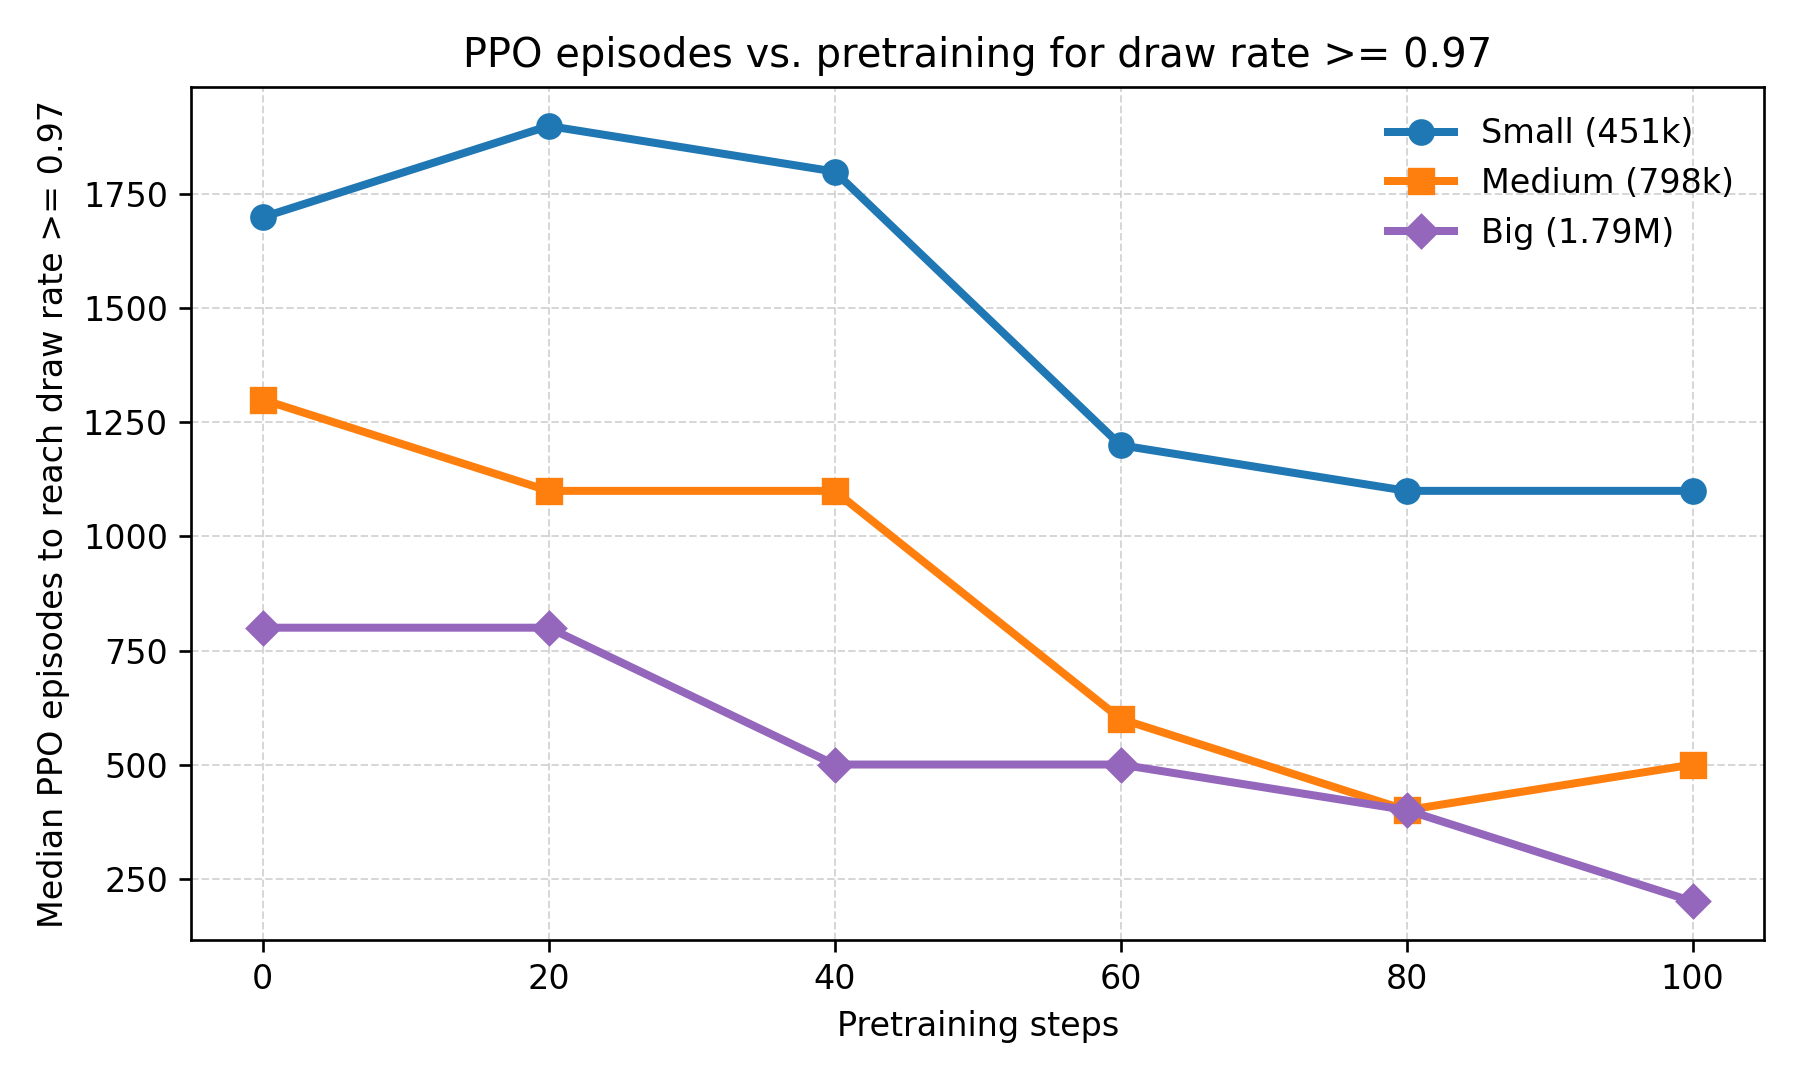
\includegraphics[width=0.75\linewidth]{warm-start-episodes-0_97.png}
    \caption{Median PPO episodes required to sustain a 0.97 draw rate as a function of supervised pretraining steps for the three model scales. Larger policies convert deeper warm starts into 3--4$\times$ sample-efficiency gains, while the small model plateaus.}
    \label{fig:episodes97}
\end{figure}

\section{Raising the Bar to a \texorpdfstring{$0.99$}{0.99} Draw Rate}
Figure~\ref{fig:episodes99} tightens the target to 0.99 draws. Short warm starts can slow PPO: the medium model needs about 2{,}200 episodes after 20 supervised steps versus 1{,}700 with no pretraining, and the big policy regresses from roughly 1{,}100 to 1{,}300 episodes in the same regime. Once the curriculum stretches to 80--100 steps, both larger models settle inside the 4{,}000-episode budget, while the small policy tops out near 1{,}800 episodes and never enters the sub-1{,}000 region.

\begin{figure}[H]
    \centering
    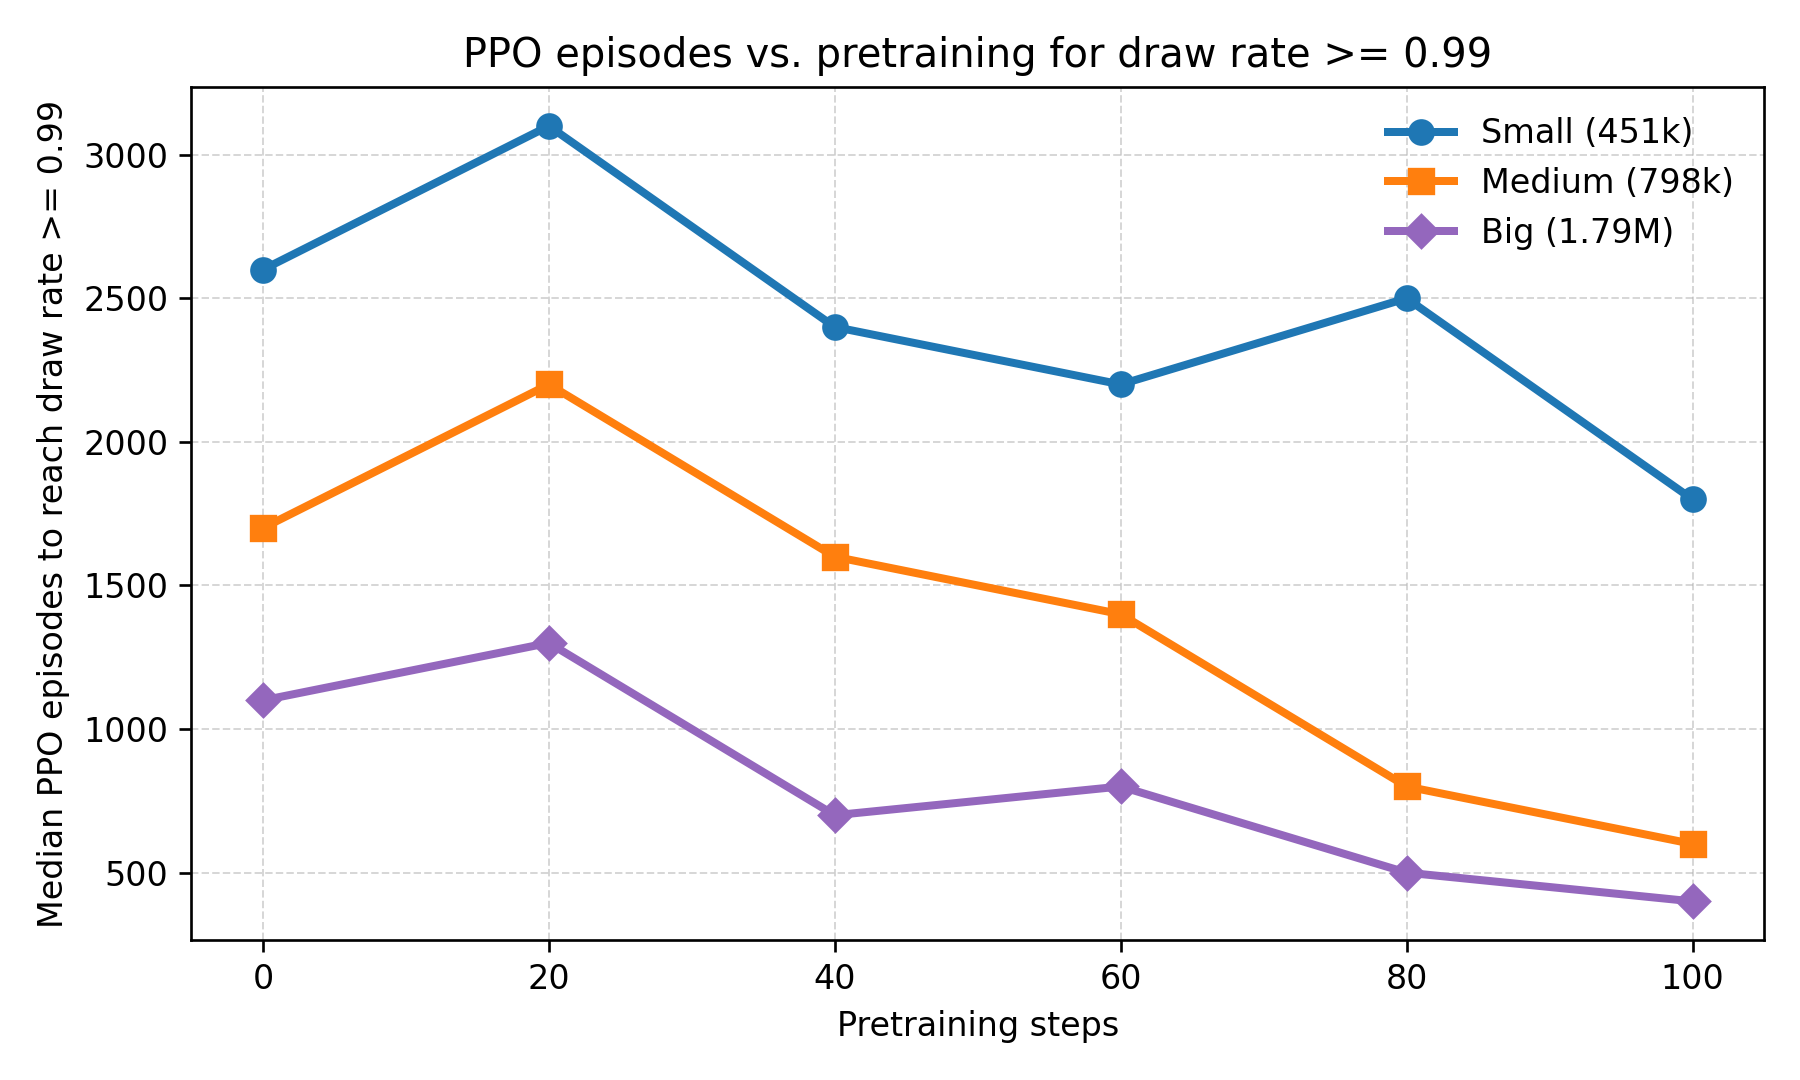
\includegraphics[width=0.75\linewidth]{warm-start-episodes-0_99.png}
    \caption{Median PPO episodes required to sustain a 0.99 draw rate. Warm starts shorter than roughly 60 steps can slow learning, while deeper curricula unlock consistent gains for the medium and big policies.}
    \label{fig:episodes99}
\end{figure}

In short, pretraining only accelerates PPO after it clears a fidelity threshold. To the left of that threshold the partially trained policies struggle to match the cold-start baseline; to the right they unlock large reductions in interaction cost.

\section{A Log-Quadratic Scaling Relationship}
Aggregating all seeds and curricula reveals a smooth relationship between the supervised loss $L$ and the PPO episodes $E$ needed to reach the 0.97 draw target. The data fit a single log-quadratic curve across capacities:
\begin{equation}
\log E = -0.147\,(\log L)^2 - 0.0066\,\log L + 7.21.
\label{eq:logquadratic}
\end{equation}

The curve captures the sharp early gains from improving the warm start and the plateau that arrives once the policy approaches its capacity floor. Its concave shape in log--log space suggests the frontier is an empirical blend of low-capacity and high-capacity regimes rather than the Taylor expansion of a single saturating power law. Even so, it still offers a concrete budgeting rule: shrinking the supervised loss from 40 to 60 steps predicts a drop from about 1{,}050 to 800 episodes, while stretching from 80 to 100 steps only buys another $\sim$270 episodes.

\begin{figure}[H]
    \centering
    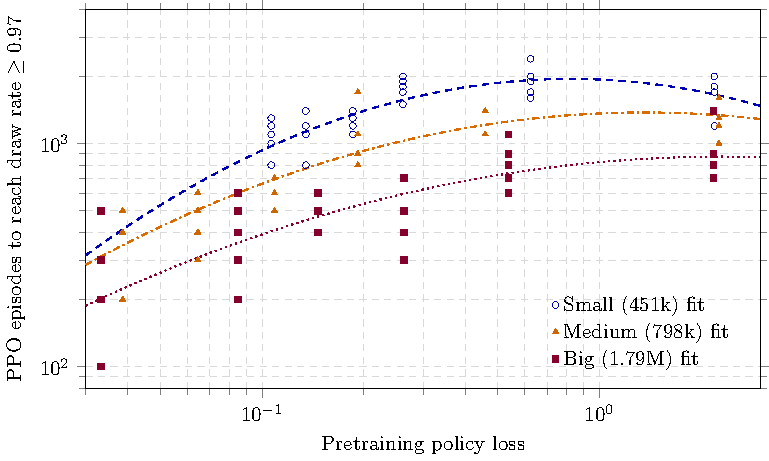
\includegraphics[width=0.75\linewidth]{warm-start-loss-frontier.pdf}
    \caption{Log-quadratic frontier linking supervised loss to PPO episodes across the small (451k parameters), medium (798k), and big (1.79M) policies. All 90 configurations fall on the same curve.}
    \label{fig:logquadratic}
\end{figure}

\section{Key Findings}
\begin{itemize}
    \item \textbf{Bigger models benefit more.} The medium and big transformers realize three-to-four-fold PPO savings once their warm starts reach 80--100 steps; the small model remains bottlenecked.
    \item \textbf{Too little pretraining can hurt.} Curricula that stop around 20 steps can increase the PPO budget at the strict 0.99 draw threshold.
    \item \textbf{Pretraining loss is a budgeting knob.} The log-quadratic frontier maps supervised loss directly to the remaining interaction budget, clarifying when to invest in more pretraining versus more RL.
\end{itemize}

\section{Implications for LLM Training}
Frontier LLM teams face the same trade-off: RLVR budgets only shrink when the model retains expressive headroom. The log-quadratic frontier suggests tracking supervised loss to decide when to switch from imitation to RLVR, and it highlights that widening the model can shift the curve more than extending a mid-fidelity curriculum. High-quality warm starts matter, but they only pay off if the policy can still absorb the signal.

\section{Limitations and Open Questions}
These conclusions stem from five seeds per configuration, a single deterministic opponent, and transformer policies orders of magnitude smaller than frontier LLMs. The warm starts are trained on flawless minimax targets; introducing label noise or partial credit could move the fidelity threshold. Scaling model size, curriculum depth, and environment complexity would test whether the same capacity-conditioned frontier holds for harder RLVR tasks such as coding and long-horizon planning.

\section*{Acknowledgements}
Thanks to Sholto Douglas for pointing me to Will Brown's tweet, which inspired this study.

\end{document}
